\begin{frame}{Theories Evolve}
  Theories are not set in stone—new evidence refines and improves them 
  over time.

  \vspace{0.5cm}

  \begin{figure}
    \centering
    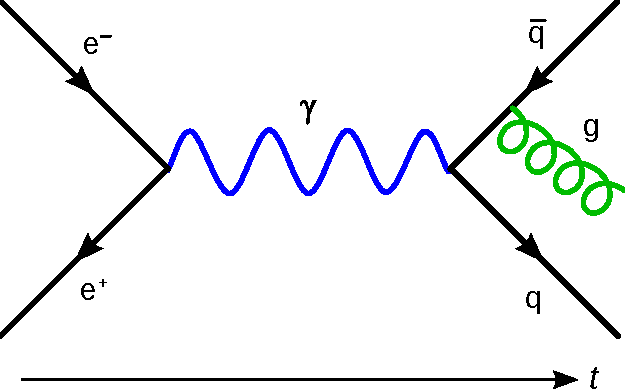
\includegraphics[width=0.7\textwidth]{Figures/Feynmann_Diagram_Gluon_Radiation.pdf}
    \caption{Quantum Field Theory, one of the most successful theories. 
    \cite{Holdsworth2007}}
  \end{figure}
\end{frame}

\begin{frame}{Principle of Parsimony}
  The simplest explanation is preferable.

  \vspace{0.5cm}
  \textbf{Example: Renormalization in Quantum Field Theory}

  Instead of introducing an infinite number of parameters, 
  renormalization allows QFT to explain physical phenomena using 
  only a few experimentally determined constants. 

  \vspace{0.5cm}
  The success of the \textbf{Standard Model} lies in its parsimony: 
  a limited set of symmetries and fundamental interactions describes 
  a vast array of experimental results.
\end{frame}

\begin{frame}{Peer Review is not Absolute}
  While it helps ensure better research, peer review has limitations—
  it can become a barrier to knowledge or create a false sense of quality.

  \vspace{0.5cm}
  \textbf{Example: Reinvention of Calculus in 1994}

  A peer-reviewed medical paper unknowingly reinvented the 
  \textbf{trapezoidal rule} for numerical integration, illustrating how 
  errors can persist in published research. \cite{Tai1994}
\end{frame}

\begin{frame}{Example: Reinvention of Calculus}
  \begin{figure}
    \centering
    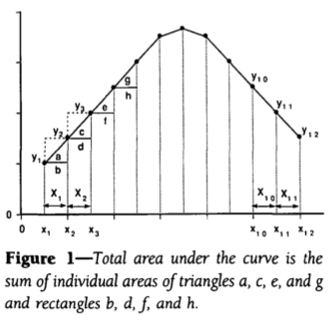
\includegraphics[width=0.7\textwidth]{Figures/calculus.png}
    \vspace{-0.25cm}
    \caption{Taken from paper. \cite{Tai1994}}
  \end{figure}
\end{frame}
